\chapter{Stage 4 --- Photometry, Pupil Dynamics, and Full Acuity Pipeline}
\label{ch:stage4}

Stage 4 (\texttt{stage4\_human\_vision/}) is the most complete acuity pipeline in this
project: it adds a real natural-pupil model and troland-based retinal photometry on
top of Stage 3's optical-quality metrics, then applies the recommended acuity route of
Chapter~\ref{ch:acuity_models}.

\section{Watson--Yellott pupil model}

Natural pupil diameter is modeled via the Watson \& Yellott (2012) unified formula,
itself built on the Stanley--Davies luminance-dependent baseline
$D_{ref}(\phi)$ (a saturating power-law in effective corneal flux density $\phi$) with
an age-dependent slope correction:
\begin{align}
\phi &= L_{scene}\cdot A_{field}\cdot(\text{monocular/binocular attenuation}) \\
D_{ref}(\phi) &= D_{max} - D_{span}\cdot\frac{r}{r+D_{offset}}, \qquad r=\left(\frac{\phi}{\phi_0}\right)^{p} \\
D(\phi, \text{age}) &= D_{ref}(\phi) + (\text{age}_{eq}-20)\cdot\big(a_0 - a_1 D_{ref}(\phi)\big)
\end{align}
clipped to the model's physiological minimum/maximum diameter. This is the same
natural pupil that determines both relative illuminance (Chapter~\ref{ch:stage3a}) and
--- via a fixed-point iteration --- the eye's actual adapted state under a given
pinhole.

\section{Retinal photometry and the pupil--illuminance coupling}

Retinal illuminance (trolands) is $\text{Td}=L_{scene}\times A_{aperture,mm^2}$
(Equation~\ref{eq:troland}), using the \emph{limiting} aperture stop (pinhole, when
smaller than the natural pupil --- true at every aperture tested in this report). Stage
4's genuinely new capability, not present in Stage 3, is a fixed-point iteration
coupling the natural pupil's own size back to the \emph{retinal} illuminance the
pinhole actually delivers (not the raw scene luminance): the pupillary light reflex
responds to actual retinal flux, which a persistent pinhole genuinely reduces. This
construction is a first-principles feedback definition, not itself drawn from a single
cited paper (Watson \& Yellott is cited for pupil-diameter-given-luminance, not for
this specific feedback loop) --- stated explicitly, not left implicit.

\subsection*{Headline finding: pinhole restriction alone crosses photopic into mesopic}

\begin{table}[htbp]
\centering
\begin{tabular}{lrrr}
\toprule
Aperture & Scene $10{,}000\,\text{cd/m}^2$ & Scene $1000\,\text{cd/m}^2$ & Scene $100\,\text{cd/m}^2$ \\
\midrule
$75\um$   & $1.50\,\text{cd/m}^2$ (mesopic)  & $0.11\,\text{cd/m}^2$ (mesopic) & $0.010\,\text{cd/m}^2$ (mesopic) \\
$400\um$  & $115.3\,\text{cd/m}^2$ (photopic) & $5.4\,\text{cd/m}^2$ (mesopic)  & $0.35\,\text{cd/m}^2$ (mesopic) \\
$2000\um$ & $6779\,\text{cd/m}^2$ (photopic)  & $395\,\text{cd/m}^2$ (photopic) & $17.6\,\text{cd/m}^2$ (photopic) \\
\bottomrule
\end{tabular}
\caption{Modeled equivalent adapting luminance, $M=4\,$D, at three scene luminances (headline Stage 4 finding).}
\label{tab:photopic-mesopic}
\end{table}

Even at the brightest scene luminance tested ($10{,}000\,\text{cd/m}^2$, unambiguously
photopic), a small enough pinhole ($75$--$150\um$) drives the modeled equivalent
adapting luminance into the mesopic range ($<\sim3\,\text{cd/m}^2$) purely through
aperture restriction. Read the reported ``natural pupil diameter'' as this model's
self-consistent equilibrium value for \emph{continuous wear} of one exact pinhole, not
as an instantaneous room-light pupil size.

\section{Full sweep: predicted logMAR, VSOTF, and illuminance}

\begin{figure}[htbp]
\centering
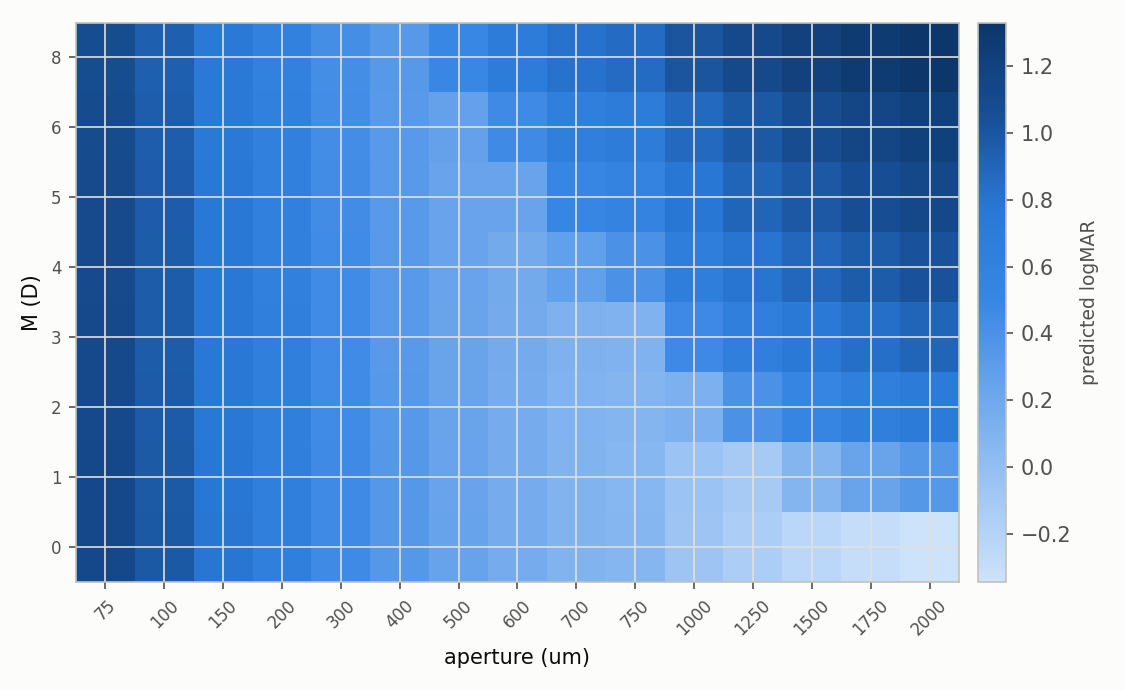
\includegraphics[width=0.85\textwidth]{figures/fig_stage4_logmar_heatmap.png}
\caption{Stage 4 predicted logMAR across the full aperture $\times$ myopia grid, $10{,}000\,\text{cd/m}^2$ scene.}
\label{fig:stage4-logmar}
\end{figure}

{\small
\begin{longtable}{rrrrr}
\caption{Aperture minimizing predicted logMAR, per myopia level (10000 cd/m2 scene).}\label{tab:stage4-full}\\
\toprule
M (D) & best-logMAR aperture (um) & logMAR & VSOTF & retinal illuminance (Td) \\
\midrule
\endfirsthead
\multicolumn{5}{c}{\tablename\ \thetable\ -- continued}\\
\toprule
M (D) & best-logMAR aperture (um) & logMAR & VSOTF & retinal illuminance (Td) \\
\midrule
\endhead
\bottomrule
\endfoot
0.000 & 2000.000 & -0.344 & 1.000 & 31415.927 \\
1.000 & 1250.000 & -0.120 & 0.831 & 12271.846 \\
2.000 & 750.000 & 0.076 & 0.867 & 4417.865 \\
3.000 & 750.000 & 0.112 & 0.726 & 4417.865 \\
4.000 & 600.000 & 0.181 & 0.760 & 2827.433 \\
5.000 & 600.000 & 0.240 & 0.649 & 2827.433 \\
6.000 & 500.000 & 0.259 & 0.709 & 1963.495 \\
8.000 & 400.000 & 0.331 & 0.739 & 1256.637 \\
\end{longtable}
}

Two secondary findings, both previously documented and reconfirmed here: (1) predicted
logMAR \emph{improves} with higher $M$ at fixed aperture, an inherited effect of the
cycles/\textmu m $\to$ cycles/degree conversion (a longer myopic eye maps the same
physical retinal blur to fewer degrees of visual angle) --- not a claim that more
myopia genuinely helps acuity, simply a unit-conversion artifact of a fixed physical
blur radius; (2) VSOTF/Strehl exceeding $1.0$ at high $M$, the same near-field
oscillation already documented in Chapter~\ref{ch:mtf_strehl}, more visible here
because VSOTF amplifies whatever the underlying OTF ratio does.
